%%This is a very basic article template.
%%There is just one section and two subsections.
\newif\ifdraft
\draftfalse
\documentclass[en,twoside,onehalfspacing,phd]{risethesis}
\usepackage[english]{babel}
\usepackage[utf8]{inputenc}
\usepackage[T1]{fontenc}
\usepackage{colortbl}
\usepackage{color}
\usepackage{graphicx}
\usepackage{epstopdf}
\usepackage{amsmath}
\usepackage{cspsymb}
\usepackage[table]{xcolor}
\usepackage{microtype}
\usepackage{bibentry}
\usepackage{subfigure}
\usepackage{multirow}
\usepackage{rotating}
\usepackage{booktabs}
\usepackage{pdfpages}
\usepackage{caption}
\usepackage{lipsum}
\def\mytitle{[TBD]}
\def\me{Andr\'{e} Lu\'{i}s Ribeiro Didier}
\usepackage[linkcolor=black,
            citecolor=blue,
            urlcolor=black,
            colorlinks,
            pdfpagelabels,
            pdftitle={\mytitle},
            pdfauthor={\me}]{hyperref}
\usepackage{cleveref}
\usepackage{etoolbox}
\usepackage{hazard-management}
\usepackage{amsthm}
\usepackage{tikz}
%\usepackage{fault-modelling-theory/generated/document/isabelle}
%\usepackage{fault-modelling-theory/generated/document/isabellesym}

\DeclareGraphicsExtensions{.pdf,.eps,.png}
\graphicspath{{./figures/}{./}}

\usetikzlibrary{positioning,arrows,shapes}
\tikzset{>=stealth'}

\captionsetup[table]{position=top,justification=centering,width=.85\textwidth,labelfont=bf,font=small}
\captionsetup[lstlisting]{position=top,justification=centering,width=.85\textwidth,labelfont=bf,font=small}
\captionsetup[figure]{position=bottom,justification=centering,width=.85\textwidth,labelfont=bf,font=small}

%% Remove colors from hyperlinks
\makeatletter
\AtBeginDocument{%
  \renewcommand*{\AC@hyperlink}[2]{%
    \begingroup
      \hypersetup{hidelinks}%
      \hyperlink{#1}{#2}%
    \endgroup
  }%
}
\makeatother

\address{Recife}

\universitypt{Universidade Federal de Pernambuco}
\universityen{Federal University of Pernambuco}

\departmentpt{Centro de Informática}
\departmenten{Center of Informatics}

\programpt{Pós-graduação em Ciência da Computação}
\programen{Graduate in Computer Science}

\majorfieldpt{Ciência da Computação}
\majorfielden{Computer Science}

\title{\mytitle}
\date{December 2014}

\author{\me}
\adviser{Alexandre Cabral Mota}
\coadviser{Alexander Romanovsky}

\newtheorem{definition}{Definition}
\newtheorem{lemma}{Lemma}
\newtheorem{theorem}{Theorem}

\ifdraft
\includeonly{introduction,temporal-fault-trees,fault-modelling}
%\includeonly{formalisation}
\fi
%%%%% Temporal gates
\newcount\pgateexp
\newcommand{\gateexp}[1]{\ifnum\the\pgateexp > 1 (#1) \else #1 \fi}

\newcommand{\OR}[2]{\advance\pgateexp 1\ensuremath{\gateexp{#1+#2}}\advance\pgateexp -1}
\newcommand{\AND}[2]{\advance\pgateexp 1\ensuremath{\gateexp{#1.#2}}\advance\pgateexp -1}
\newcommand{\POR}[2]{\advance\pgateexp 1\ensuremath{\gateexp{#1|#2}}\advance\pgateexp -1}
\newcommand{\PAND}[2]{\advance\pgateexp 1\ensuremath{\gateexp{#1<#2}}\advance\pgateexp -1}
\newcommand{\SAND}[2]{\advance\pgateexp 1\ensuremath{\gateexp{#1\&#2}}\advance\pgateexp -1}
\newcommand{\SV}{\ensuremath{\mathrm{SV}}}
\newcommand{\SVtuple}[1][n]{\ensuremath{\underbrace{\SV \cross \ldots \cross \SV}_{#1}}}

\newcommand{\powerset}{\ensuremath{\mathcal P}}

%%%%% Boolean gates
\newcommand{\BOR}[2]{#1\mathrm{+^B}#2}



%%%% Abbreviations

%TODO
\newcommand{\TODO}[1]{{\color{red}\relsize{+1}TODO: #1}}

\newcommand{\nat}{\ensuremath{\mathbb{N}}}


\newcommand{\newabbrevdescr}[2]{%
\expandafter\newif\csname if#1CHECK\endcsname%
\expandafter\newcommand\csname #1presentation\endcsname{#1}%
\expandafter\newcommand\csname #1expanded\endcsname{#2\global\csname#1CHECKtrue\endcsname}%
\expandafter\newcommand\csname #1\endcsname{%
  \csname if#1CHECK\endcsname%
  \csname #1presentation\endcsname%
  \else
  \csname #1expanded\endcsname~(\csname #1presentation\endcsname)%
  \fi%
\xspace}%
}

\newcommand{\renewabbrevdescr}[2]{%
\expandafter\newif\csname if#1CHECK\endcsname%
\expandafter\newcommand\csname #1presentation\endcsname{#1}%
\expandafter\newcommand\csname #1expanded\endcsname{#2\global\csname #1CHECKtrue\endcsname}%
\expandafter\renewcommand\csname #1\endcsname{%
  \csname if#1CHECK\endcsname%
  \csname #1presentation\endcsname
  \else
  \csname #1expanded\endcsname
  \fi%
\xspace
}%
}

\newcommand{\newabbrevdescrext}[3]{%
\expandafter\newcommand\csname #2\endcsname{%
  \csname if#1CHECK\endcsname%
  #2
  \else
  #3\expandafter\csname #1CHECKtrue\endcsname
  \fi%
\xspace
}%
}

\newabbrevdescr{CSP}{Communicating Sequential Processes}
\renewabbrevdescr{CSPM}{Machine-readable version of \CSP}
\renewcommand\CSPMpresentation{\CSP{$_M$}}

\newabbrevdescr{TTT}{Temporal Truth Table}
\newabbrevdescrext{TTT}{TTTs}{Temporal Truth Tables}

\newabbrevdescr{TFT}{Temporal Fault Tree}
\newabbrevdescrext{TFT}{TFTs}{Temporal Fault Trees}

\newabbrevdescr{FT}{Fault Tree}
\newabbrevdescrext{FT}{FTs}{Fault Trees}

\newabbrevdescr{CDHAT}{Conceptual design hazard analysis type}
\renewcommand{\CDHATpresentation}{CD-HAT}
\newabbrevdescr{PDHAT}{Preliminary design hazard analysis type}
\renewcommand{\PDHATpresentation}{PD-HAT}
\newabbrevdescr{DDHAT}{Detailed design hazard analysis type}
\renewcommand{\DDHATpresentation}{DD-HAT}
\newabbrevdescr{SDHAT}{System design hazard analysis type}
\renewcommand{\SDHATpresentation}{SD-HAT}
\newabbrevdescr{ODHAT}{Operations design hazard analysis type}
\renewcommand{\ODHATpresentation}{OD-HAT}
\newabbrevdescr{HDHAT}{Health design hazard analysis type}
\renewcommand{\HDHATpresentation}{HD-HAT}
\newabbrevdescr{RDHAT}{Requirements design hazard analysis type}
\renewcommand{\RDHATpresentation}{RD-HAT}

\newabbrevdescr{PHL}{Preliminary Hazard List}
\newabbrevdescr{PHA}{Preliminary Hazard Analysis}
\newabbrevdescr{SSHA}{Subsystem Hazard Analysis}
\newabbrevdescr{SHA}{System Hazard Analysis}
\newabbrevdescr{OSHA}{Operating and Support Hazard Analysis}
\renewcommand{\OSHApresentation}{O\&SHA}
\newabbrevdescr{HHA}{Health Hazard Assessment}
\newabbrevdescr{SRCA}{Safety Requirements/Criteria Analysis}
\newabbrevdescr{FTA}{Fault Tree Analysis}
\newabbrevdescr{ETA}{Event Tree Analysis}
\newabbrevdescr{FMEA}{Failure Mode and Effects Analysis}
\newabbrevdescr{FaHA}{Fault Hazard Analysis}
\newabbrevdescr{FuHA}{Functional Hazard Analysis}
\newabbrevdescr{SCA}{Sneak Circuit Analysis}
\newabbrevdescr{SWSCA}{}
\newabbrevdescr{PNA}{Petri Net Analysis}
\newabbrevdescr{MA}{Markov Analysis}
\newabbrevdescr{BA}{Barrier Analysis}
\newabbrevdescr{HAZOP}{Hazard and Operability Analysis}
\newabbrevdescr{CCA}{Cause--Consequence Analysis}
\newabbrevdescr{CCFA}{Common Cause Failure Analysis}
\newabbrevdescr{MORT}{Management Oversight Risk Tree Analysis}
\newabbrevdescr{SWHA}{Software Safety Assessment}
\newabbrevdescr{BPA}{Bent Pin Analysis}
\newabbrevdescr{THA}{Threat Hazard Assessment}


\begin{document}

\ifdraft\else
\frontmatter
\frontpage
\presentationpage

\begin{fichacatalografica}
  \FakeFichaCatalografica % Comment this line when you have the correct file
%     \includepdf{ficha_catalografica.pdf} % Uncomment this
\end{fichacatalografica}
\banca
\begin{dedicatory}
I dedicate this thesis to Juliana, Luciana and Snowflake.
\end{dedicatory}

\acknowledgements
I would like to thank to the following people:
\begin{enumerate}
  \item Alexandre
  \item Sascha
  \item Augusto Sampaio
  \item Zoe
  \item John Fitz.
\end{enumerate}
\ldots

\begin{epigraph}[title]{author}
[Text]\\
\vspace{0.5cm}
[More text\ldots]
\end{epigraph}
\fi

\resumo
Resumo\ldots
\begin{keywords}
\end{keywords}

\abstract
Abstract\ldots
\begin{keywords}
\end{keywords}


\ifdraft\else
\listoffigures
\listoftables
% Acronyms manual: http://linorg.usp.br/CTAN/macros/latex/contrib/acronym/acronym.pdf
\listofacronyms
%
\ExplSyntaxOn
% this now only works because I've use the same already in the preamble so
% it does nothing here:
\ProvideAcroEnding {possessive} {'s} {'s}

\ProvideAcroCommand \acg
{
	\acro_possessive:
	\acro_use:n {#1}
}
\NewAcroCommand \acgp
{
	\acro_possessive:
	\acro_plural:
	\acro_use:n {#1}
}

\NewAcroCommand \acsg
{
	\acro_possessive:
	\acro_short:n {#1}
}

\NewAcroCommand \theac
{
	\acro_if_acronym_used:nTF {#1}{}{the\xspace}
	\acro_use:n {#1}
}

\ExplSyntaxOff

\DeclareAcronym{algebra}{%
	short=ATF,
	long=Algebra of Temporal Faults
}

\DeclareAcronym{activation}{%
	short=ActA,
	long=Activation Algebra
}

\DeclareAcronym{BDD}{%
	short=BDD,
	long=Binary Decision Diagram,
	cite={{Akers1978,Boute1976}}
}

\DeclareAcronym{csp}{%
	short=CSP,
	long=Communicating Sequential Processes,
	cite={Roscoe1997}
}

\DeclareAcronym{CSp}{%
	short=CSp,
	long=\acsg*{DFT} cold spare gate
}

\DeclareAcronym{cspm}{%
	short=CSP{$_M$},
	long=Communicating Sequential Processes
}
%\acropost{cspm}{\footnote{This variant ``M'' is the machine-readable version of \acs{csp}.}}

\DeclareAcronym{DFT}{%
	short=DFT,
	long=Dynamic Fault Tree,
	cite={DBB1992}
}

\DeclareAcronym{fba}{%
	short=FBA,
	long=Free Boolean Algebra,
	cite={[pp. 256-266]{GH2009}}
}

\DeclareAcronym{FDEP}{%
	short=FDEP,
	long=\acsg*{DFT} functional dependency gate
}

\DeclareAcronym{fdr}{%
	short=FDR,
	long=Failures and Divergences Refinement,
	short-indefinite=an
}

\DeclareAcronym{FTA}{%
	short=FTA,
	long=Fault Tree Analysis,
	short-indefinite=an
}

\DeclareAcronym{SEQ}{%
	short=SEQ,
	long=\acsg*{DFT} sequence enforcing gate
}

\DeclareAcronym{SFT}{%
	short=SFT,
	long=Static Fault Tree,
	short-indefinite=an
}

\DeclareAcronym{TFT}{%
	short=TFT,
	long=Temporal Fault Tree,
	cite={WP2008,WP2009}
}

\DeclareAcronym{hiphops}{%
	short=HiP-HOPS,
	long=Hierarchically Performed Hazard Origin and Propagation Studies,
	cite={PMS+2001}
}

%\acresetall
%\end{acronym}
%\lstlistoflistings
\fi
\tableofcontents

\mainmatter

\chapter{Introduction}

\begin{quotation}[Título]{Autor}
Texto \\
Text
\end{quotation}

\noindent OLD:\{
\begin{enumerate}
  \item Reliability engineering
  \begin{enumerate}
    \item Describe safety (related to lives), reliability (related to cost).
  \end{enumerate}
  \item Fault tolerance
  \begin{enumerate}
    \item Definition
    \item Patterns
  \end{enumerate}
  \item Functions to describe component behaviour. Include time
  \item Make a ft-pattern replaceable by its function refinement.
\end{enumerate}
\}

%\usepackage{graphics} is needed for \includegraphics
\begin{figure}[htp]
\begin{center}
  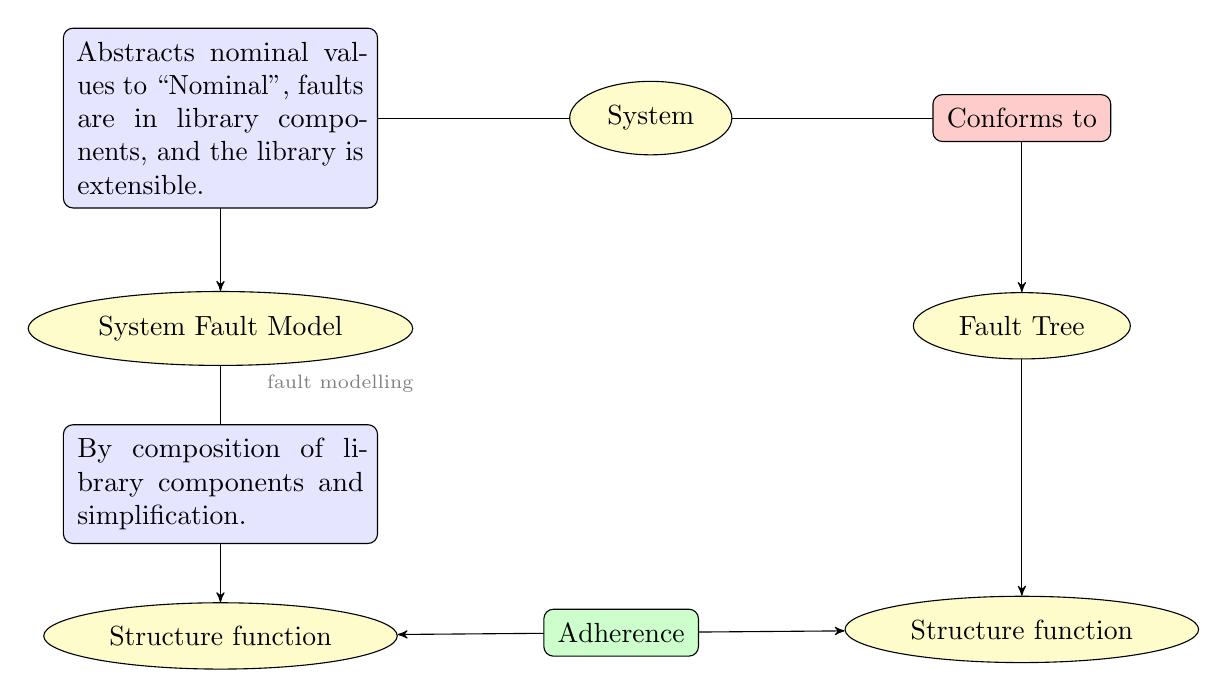
\begin{tikzpicture}[
block/.style={ellipse, draw, fill=yellow!20, rounded corners=.8ex, inner sep=5pt},
edgedesc/.style={rectangle, draw, fill=blue!10, rounded corners=.8ex, inner sep=5 pt},
every label/.style={gray, font=\scriptsize}
]
\node (system) [block] {System};
\node (faultmodel) [block, below left=2cm and 3cm of system, label={below right: fault modelling}] {System Fault Model};
\node (structurefSFM) [block, below=3cm of faultmodel] {Structure function};
\node (faulttree) [block, below right=2cm and 3cm of system] {Fault Tree};
\node (structurefFT) [block, below=3cm of faulttree] {Structure function};


\draw [->] (system) -| node[edgedesc] {%
\begin{minipage}{0.3\textwidth}
Abstracts nominal values to ``Nominal'', faults are in library components, and the library is extensible.
\end{minipage}
} (faultmodel);
\draw [->] (system) -| node[edgedesc, fill=red!20] {Conforms to} (faulttree);
\draw [->] (faultmodel) -- node[edgedesc] {%
\begin{minipage}{0.3\textwidth}
By composition of library components and simplification.
\end{minipage}
} (structurefSFM);
\draw [->] (faulttree) -- (structurefFT);
\draw [<->] (structurefSFM) -- node [edgedesc, fill=green!20] {Adherence} (structurefFT);
\end{tikzpicture}
  \caption{Overview}
  \label{fig:overview}
\end{center}
\end{figure}

\chapter{Modelling faults}
\label{sec:fault-modelling}

\begin{quotation}[Título]{Autor}
Texto \\
Text
\end{quotation}

In this section we show how to model faults using functions in a component-level failure logic.
%
We define two relations to establish our axioms: (i) failure value and failure state, (ii) order of occurrence.
%
Using these definitions we are able to create a library of basic components that can be used as building blocks to create new components or to compose a system model.

\section{Modelling a system}
\label{sec:modelling-a-system}

A system model is a block diagram (nodes) with directed connected arrows. 
%
An arrow origin is the output of some component and the destination is one or more inputs of other component.
%
Two output ports cannot be directly connected, nor does two inputs.
%
It is required an output and at least one input to connect two components.

Arrows and nodes contain fault-related information.
%
An arrow contains the current value of the output of the originating node.
%
It is a Boolean indicating a nominal or an erroneous value. 
%
In the last case, the arrow also contains the error mode.
%
A node contains: (i) state information, indicating whether the component is in failure, and (ii) a logic for each output that expresses how the output reacts to internal failures and failures on the inputs. 
%
Item (ii) is very similar to the cause of output deviation in \HIPHOPS[TODO: citar def. HH].
%
It also includes the order of occurrence of the failures.

Differently from \HIPHOPS, an output expression also contains the nominal case to cover all possibilities on the components, to avoid missing a case.

%%%%%%%%%%%%%%%%%%%%%%%%%%%%%%%%%%%%%%%%%%%%%%%%%%%%%%%%%%%%%%%%%%%%%%%%%%%%%%%%
% Failure value and failure state%%%%%%%%%%%%%%%%%%%%%%%%%%%%%%%%%%%%%%%%%%%%%%%
%%%%%%%%%%%%%%%%%%%%%%%%%%%%%%%%%%%%%%%%%%%%%%%%%%%%%%%%%%%%%%%%%%%%%%%%%%%%%%%%
\subsection{Failure value and failure state}

A function $F_i : Input \rightarrow Boolean$ expresses whether the current value on an input is a failure value. 
%
Similarly, a function $F_c : Component \rightarrow Boolean$ expresses whether the current state of a component is a failure state.
%
The type of a failure value is defined by a unbounded value.

To illustrate these definitions, suppose a component $C$ that contains only one output and its failure logic depends only on its internal state: if it is faulty, it produces an omission value $O_M$, otherwise it produces a nominal value $N$. 
%
The failure logic for its output $O$ is: $O = F_c(C) \land O_M \lor \lnot F_c(C) \land N$.

\subsection{Order of occurrence}

The order of occurrence of events is defined as a sequence value as it is in \HIPHOPS: it is a natural value assigned to each input.
%
The value does not contain gaps, so always there is a pair of input that the modulus of the difference of their sequence values is 1, or the modulus of the difference is 0 for all pairs of inputs.
%
For example, if we have two variables, they can be assigned values 0 and 1 or 1 and 2, but not 0 and 2. 

We define a relation $S : Input \rightarrow \nat $ as the sequence value for the given input.

\chapter{Temporal Fault Trees}
\label{sec:tft}

\begin{quotation}[Título]{Autor}
Texto \\
Text
\end{quotation}

Compared to traditional \FTs, \TFTs can describe the order of occurrence of events. A specific order of occurrence causes a top event, thus the concept of failure expressions is augmented. Instead of using traditional Boolean gates, they use special gates named temporal gates (see \cref{tab:temporal-gates}). They differ on what kind of input they compare: Boolean gates compare Boolean values whilst temporal gates compare \emph{sequence values}. A sequence value is a natural number in which each basic event happens on a specific value, but there are no gaps on the sequence (see \cref{tab:temporal-gates-sv-formulas}). Zero values indicate that the event has not happened. As in Boolean logic, temporal logic also has truth tables, which are named \TTTs.

\TFTs can be written as an expression where each basic event in a tree is a variable in the expression. \Cref{tab:temporal-gates-ttt} shows a \TTT---a result of direct application of the equations shown in \cref{tab:temporal-gates-sv-formulas}---for each temporal gate basic formula, using events A and B. 

\begin{table}
\caption{Temporal gates}
\label{tab:temporal-gates}
\center
\begin{tabular}{|l|c|c|p{6cm}|}
\hline
\textbf{Name} & \textbf{Abbrev.} & \textbf{Operator} & \textbf{Description}\\
\hline
\hline
Or & OR & + & Similarly to the Boolean operator, whenever one of its inputs is higher than $0$, it outputs its value.\\
\hline
And & AND & . & When both inputs are higher than zero, it outputs the value of the maximum sequence value.\\
\hline
Priority Or& POR & | & When the first input is higher than zero, it outputs its value and the second output may or may not occur. It will not output a value when only the second output is higher than the first output.\\
\hline
Priority And & PAND & < & It outputs the value of the second output if the first output occurs strictly before the second.\\
\hline
Synchronous And & SAND & \& & It outputs the value of the sequence value when both inputs occur.\\
\hline
\end{tabular}
\end{table}

\begin{table}
\caption{Sequence value (SV) equations for each temporal gate}
\label{tab:temporal-gates-sv-formulas}
\center
\begin{tabular}{|c|l|}
\hline
\textbf{Gate} & \textbf{Sequence value formula} \\
\hline
\hline
OR & $\SV(\OR{A}{B}) = \left\{
\begin{array}{ll}
  \min(\SV(A), \SV(B)) &, \SV(A) > 0 \land \SV(B) > 0\\
  \max(\SV(A), \SV(B)) & \text{otherwise}
\end{array}
\right.$\\
\hline
AND & $\SV(\AND{A}{B}) = \left\{
\begin{array}{ll}
  \max(\SV(A), \SV(B)) &, \SV(A) > 0 \land \SV(B) > 0\\
  0 & \text{otherwise}
\end{array}
\right.$\\
\hline
POR & $\SV(\POR{A}{B}) = \left\{
\begin{array}{ll}
  \SV(A) &, \SV(B) = 0 \lor \SV(A) < \SV(B) \\
  0 & \text{otherwise}
\end{array}
\right.$\\
\hline
PAND & $\SV(\PAND{A}{B}) = \left\{
\begin{array}{ll}
  \SV(B) &, \SV(A) > 0 \land \SV(A) < \SV(B) \\
  0 & \text{otherwise}
\end{array}
\right.$\\
\hline
SAND & $\SV(\SAND{A}{B}) = \left\{
\begin{array}{ll}
  \SV(A) &, \SV(A) = \SV(B) \\
  0 & \text{otherwise}
\end{array}
\right.$\\
\hline
\end{tabular}
\end{table}

\begin{table}
\caption{\TTT for each temporal gate}
\label{tab:temporal-gates-ttt}
\center
\begin{tabular}{|c|c|c|c|c|c|c|}
\hline
\textbf{A} & \textbf{B} & {$\OR{A}{B}$} & $\AND{A}{B}$ & $\POR{A}{B}$ & $\PAND{A}{B}$ & $\SAND{A}{B}$ \\
\hline
\hline
0 & 0 & 0 & 0 & 0 & 0 & 0\\
0 & 1 & 1 & 0 & 0 & 0 & 0\\
1 & 0 & 1 & 0 & 1 & 0 & 0\\
1 & 1 & 1 & 1 & 1 & 0 & 1\\
1 & 2 & 1 & 2 & 1 & 2 & 0\\
2 & 1 & 1 & 2 & 0 & 0 & 0\\
\hline
\end{tabular}
\end{table}

\section{Formalisation of Temporal Fault Trees}
\label{sec:tft-formalisation}

In this section, I propose a formalisation in \CSP of \TFT to enable a comparison of \TFTs and the calculation of the probability of occurrence of top events.

The formalisation occurs in three steps: (i) formalising sequence values calculations to achieve \TTTs for a given temporal expression (\cref{sec:sv-calculus}), (ii) converting these \TTTs to sequences of events (\cref{sec:ttt-to-seqs}), and (iii) building a process to call these events to verify refinements (\cref{sec:seqs-to-process}).

\subsection{Sequence Value Calculus}
\label{sec:sv-calculus}

Given two sequence values as inputs, each temporal gate expression is encoded as a \CSP function as following:
\begin{align}
OR(a,b) & = 
  \begin{cases}
  min(a,b) & \text{if } a > 0 \land b > 0\\
  max(a,b) & \text{otherwise}
  \end{cases}\\
AND(a,b) & =
  \begin{cases}
  max(a,b) & \text{if } a > 0 \land b > 0\\
  0 & \text{otherwise}
  \end{cases}\\ 
POR(a,b) & =
  \begin{cases}
  a & \text{if } a > 0 \land (b = 0 \lor a < b)\\
  0 & \text{otherwise}
  \end{cases}\\ 
PAND(a,b) & =
  \begin{cases}
  b & \text{if } a > 0 \land a < b\\
  0 & \text{otherwise}
  \end{cases}\\ 
SAND(a,b) & =
  \begin{cases}
  a & \text{if } a = b\\
  0 & \text{otherwise}
  \end{cases}
\end{align}

Combining these functions, any temporal expression can be written. For example, given the expression $\PAND{\OR{A}{B}}{C}$, it can be written as: $PAND(OR(A,B),C)$. \Cref{tab:example-expression-ttt} shows the truth table for this example formula, by applying the function definitions for each row.

\begin{table}
\caption{\TTT for the expression $\PAND{\OR{A}{B}}{C}$}
\label{tab:example-expression-ttt}
\center
{\scriptsize
\begin{tabular}{|c|c|c|c|c|}
\hline
\textbf{A} & \textbf{B} & \textbf{C} & $\OR{A}{B}$ & $\PAND{\OR{A}{B}}{C}$ \\
\hline
\hline
0 & 0 & 0 & 0 & 0\\
0 & 0 & 1 & 0 & 0\\
0 & 1 & 0 & 1 & 0\\
0 & 1 & 1 & 1 & 0\\
0 & 1 & 2 & 1 & 2\\
0 & 2 & 1 & 2 & 0\\
1 & 0 & 0 & 1 & 0\\
1 & 0 & 1 & 1 & 0\\
1 & 0 & 2 & 1 & 2\\
1 & 1 & 0 & 1 & 0\\
1 & 1 & 1 & 1 & 0\\
1 & 1 & 2 & 1 & 2\\
1 & 2 & 0 & 1 & 0\\
1 & 2 & 1 & 1 & 0\\
1 & 2 & 2 & 1 & 2\\
1 & 2 & 3 & 1 & 3\\
1 & 3 & 2 & 1 & 2\\
2 & 0 & 1 & 2 & 0\\
2 & 1 & 0 & 1 & 0\\
2 & 1 & 1 & 1 & 0\\
2 & 1 & 2 & 1 & 2\\
2 & 1 & 3 & 1 & 3\\
2 & 2 & 1 & 2 & 0\\
2 & 3 & 1 & 2 & 0\\
3 & 1 & 2 & 1 & 2\\
3 & 2 & 1 & 2 & 0\\
\hline
\end{tabular}
}
\end{table} 

\subsection{From \TTTs to sequences of events}
\label{sec:ttt-to-seqs}

Obtaining (a set of) sequences of events is an intermediate step to get a process that represents a \TFT. This step is an optimisation to remove non-determinism, trimming the paths that lead to the top-level event. It combines paths that have the same initial event, building an hierarchical structure of choices.

The function $TTT$ below creates a set o tuples of size $n+1$, where $n$ is the number of basic events on the expression and the value on position $n+1$ is the result of the application of the temporal expression:
\begin{align}
TTT & :: TExp \Longrightarrow \powerset\left(\SVtuple[n+1]\right)\nonumber\\
TTT(expression) & = \left\{ (a_1, \ldots, a_n, expression(a_1, \ldots, a_n)) \vphantom{\clause}\nonumber\right.\\
& \qquad\left.\clause (a_1, \ldots, a_n) \in TTT_{inputs}(n)) \right\}
\end{align}
\noindent where $1,\ldots,n$ are the indexes of basic events, $\SV = \left\{0,\ldots,n\right\}$ are sequence values and $TTT_{inputs}$ defines a set of tuples of size $n$ that represents the events (inputs) for each row in a \TTT:
\begin{align}
TTT_{inputs} & :: I \Longrightarrow \powerset\left(\SVtuple\right)\\
TTT_{inputs}(n) & = \left\{ (a_1, \ldots, a_n) \vphantom{\clause}\right.\nonumber\\
 & \qquad\left. \clause max(a_1,\ldots,a_n) = card\left(\left\{a_1, \ldots, a_n\right\} \setminus \left\{0\right\}\right) \right\} \label{eq:ttt-inputs}
\end{align}

\noindent where $I = \left\{1,\ldots,n\right\}$. Note that the clause $max(a_1,\ldots,a_n) = card\left(\left\{a_1, \ldots, a_n\right\} \setminus \left\{0\right\}\right)$ guarantees that there are no gaps between two $a_i$'s, satisfying the \TFT property for sequence values.

For the example expression $\PAND{\OR{A}{B}}{C}$, the functions $TTT$ and $TTT_{inputs}$ return a set with cardinality $26$.

Finally, we create a data structure to avoid non-determinism and optimise the final process creation. This data structure is created in two steps: 
\begin{enumerate}
  \item Each tuple is converted into a set of pairs recursively where the first element is an available event and the second element is a set of options of events to choose. This set of options may contain others pairs recursively.
  \begin{align}
  SoP\left(sync_{ev}, \left(a_1,\ldots,a_n\right)\right) &= 
  \end{align}
  \noindent where $sync_{ev}$ is an event that indicates that the following events occur with the same sequence value.
  \item These pairs are then merged with respect to the first element. If there two pairs with the same first element, they are merged, making a union of the second element sets. 
\end{enumerate}


\subsection{Checking process refinements}
\label{sec:seqs-to-process}

Using the tuples defined by \cref{eq:ttt-inputs}, we now define a process that represents the execution of a temporal expression.

\chapter{Formalisation of Hazard Management}

Hazard properties, extracted from~\cite{ericsonII2005}:
%
\begin{enumerate}
  \item Hazardous element (HE);
  \item Initiating mechanisms (IM): sequence of events to activate the hazard;
  \item Target and Threat (T/T): the person or system and its corresponding threat;
  \item Status: open or closed. A hazard can only be closed if it has been verified through analysis, inspection or testing that the safety requirements are implemented in the design and successfully tested for effectiveness.
  \item Mitigation: lists the recommended actions obtained by all analysis
  \begin{itemize}
    \item Eliminate through design selection;
    \item Incorporate safety devices;
    \item Provide warning devices;
    \item Develop procedures and training;
    \item Control hazard through design methods.
  \end{itemize}
  \item Mishap Risk Index (initial, current, final) -- qualitative measurement:
  \begin{itemize}
    \item Severity
    \begin{enumerate}
      \item Catastrophic;
      \item Critical;
      \item Marginal;
      \item Negligible.
    \end{enumerate}
    \item Probability
    \begin{enumerate}
      \item Frequent;
      \item Probable;
      \item Occasional;
      \item Remote;
      \item Improbable.
    \end{enumerate}
  \end{itemize} 
\end{enumerate}

Scope of system to which Hazard Analysis make sense: those that have signal, material and energy.
%
All system functional elements~\cite[p. 47]{KSS+2011} are:
\begin{itemize}
  \item Signal---generate, transmit, distribute, and receive signals used in passive or active sensing and in communications;
  \item Data---analyse, interpret, organize, query, and/or convert data and information into forms desired by the user or other systems;
  \item Material---provide system structural support or enclosure, or transform the shape, composition, or location of material substances;
  \item Energy---provide and convert energy or propulsive power to the system.
\end{itemize}

\begin{definition}[Identifier]
It can be modelled as any user-defined data type. It can be a sequence of alphanumeric symbols (a descriptive text of the element) or a natural number (for example: an identification of a system element). It is a basic data type $\hmdatatypeId$ used in other definitions.
\end{definition}

\begin{definition}[Component]
A component is any functional or physical block within a system that may contain a hazard. $\hmdatatypecomponent: \hmdatatypeId$
\end{definition}

\begin{definition}[Hazardous element]
A hazardous element represents an element that can potentially harm someone or something.
$\hmdatatypeHE: \hmdatatypeId$.
\end{definition}

\begin{definition}[Initiating mechanism]
An initiating mechanism is an event on the system.
%
$\hmdatatypeIM: \hmdatatypeId$
%it can be a CSP process. 
\end{definition}

\begin{definition}[Target/Threat]
A target and threat pair represents the person or system that is harmed if a hazardous element is activated by the initiating mechanisms and the nature of the harm. 
%
$\hmdatatypeTT: \hmcartesian{\hmdatatypeId}{\hmdatatypeId}$.
\end{definition}

\begin{definition}[Hazard]
Given a hazardous element $HE$, a sequence of $n$ initiating mechanisms $\hmseqenum{IM_1, \ldots, IM_n}$ and a target-threat pair $T/T$, a hazard $H$ is defined as: $H: \hmdatatypeId$ and is obtained by a total, bijective function $\hmhazardsymbol$: 
%
\\$\hmhazardsymbol: \hmtotalbijectivefunction{\hmcartesian{\hmcartesian{\hmdatatypeHE}{\hmdatatypeTT}}{\hmseq{\hmdatatypeIM}}}{\hmdatatypeId}$
%
\\which is written as:
%
\\$H = \hmhazard{HE}{\hmseqenum{IM_1, \ldots, IM_n}}{T/T}$.
\end{definition}

\begin{definition}[Probability function]
A probability function $\hmprobabilitysymbol$ is used to associate values to elements in the system.
%
It is defined through analysis. 
%
$\hmprobabilitysymbol: \hmpartialfunction{\hmdatatypeId}{\hmdatatypeR}$
\end{definition}

\begin{definition}[Analysis method]
An analysis method $\hmdatatypeAM$, such that $\hmdatatypeAM: \hmdatatypeId$, describes a method used to analyse an element. 
%
It is defined as an enumerated set with the following value correspondence:
%
\begin{description}
  \item[PHL] \PHL;
  \item[PHA] \PHA;
  \item[\ldots] \TODO{Add others.}
\end{description}
\end{definition}

\begin{definition}[Time]
Time $\hmdatatypetime$ is abstracted with equal and before relations. 
%
It is defined as a sequence of time tags.
%
$\hmdatatypetime: \hmseq{\hmdatatypetimetag}$.
\end{definition}

\begin{definition}[Time tag]
A time tag represents an instantaneous observation of time.
%
It is defined as an identification: $\hmdatatypetimetag: \hmdatatypeId$
\end{definition}

\begin{definition}[Analysis]
Given an analysis method $M$, such that $M: \hmdatatypeAM$, a time tag $t$, such that $t:\hmdatatypetimetag$, an element $E$, such that $E:\hmdatatypeId$, and a probability $p$, such that $p:\hmdatatypeR$, an analysis $A$ is defined as:
%
\\$A: \hmcartesian{\left(\hmcartesian{\hmdatatypeId}{\hmdatatypetimetag}\right)}{\left(\hmcartesian{\hmdatatypeAM}{\hmdatatypeR}\right)}$
%
\\$A = \left(\left(E, t\right), \left(M, p\right) \right)$

\end{definition}
The probability function is then updated accordingly to an analysis. For example, for the analysis above, the probability function $P$ can be updated as:
$\hmprobabilitysymbol = \hmoverride{\hmprobabilitysymbol}{\left\{\hmmapsto{E}{p}\right\}}$.

\begin{definition}[Hazard activation probability]
Given a probability function $\hmprobabilitysymbol$, such that $P: \hmpartialfunction {\hmdatatypeId}{\hmdatatypeR}$, a hazardous element $HE$, a sequence of $n$ initiating mechanisms $\hmseqenum{IM_1,\ldots,IM_n}$ and a target-threat pair $T/T$, the probability of the activation of the hazard $H = \hmhazard{HE}{\hmseqenum{IM_1,\ldots,IM_n}}{T/T}$ is:
%
\\$\hmprobability{H} = \hmtimes{\hmprobability{HE}}{\hmtimes{\hmtimes{\hmprobability{IM_1}}{\ldots}}{\hmprobability{IM_n}}}$
\end{definition}

\begin{definition}[Mishap]
A mishap is defined as a pair of the probability of a hazard and the severity in case it happens: $M: \hmcartesian{\hmdatatypeR}{\hmdatatypeseverity}$.
\end{definition}
%
\noindent Where $\hmdatatypeseverity$ is a finite set, such that $\hmdatatypeseverity \subset \hmdatatypeN$. It contains the following values:
\begin{description}
  \item[1] $=$ Catastrophic;
  \item[2] $=$ Critical;
  \item[3] $=$ Marginal and
  \item[4] $=$ Negligible.
\end{description}

\section{Refinement}

In this section we define a refinement relation on a hazard model of a system.

\TODO{Add definitions on the hazard model
\begin{itemize}
  \item Set of analysis;
  \item Probability function;
  \item Addition of analysis updates probability function;
\end{itemize}
}

There a few situations in which a refinement is desirable:
\begin{description}
  \item[Hazard analysis.] A hazard model is said to be an analysis of another model if at least one new analysis was added.
  \item[Hazard mitigation.] A hazard model is said to be a mitigation of another if at least one hazard is mitigated through probability decrease. If $\hmprobabilitysymbol$ is the probability function of the previous model and $\hmprobabilitysymbol'$ is the probability function of the refined model, then: 
%
$\hmforall{e \in \hmdatatypeId}{\hmprobability[\hmprobabilitysymbol']{e}\leq\hmprobability{e}}$.
\end{description}



\chapter{Related work}

\begin{quotation}[Título]{Autor}
Texto \\
Text
\end{quotation}

\section{Title}

\subsection{Subtitle}

Plain text.

\subsection{Another subtitle}

More plain text.


%\bibliographystyle{natbib}
%\addcontentsline{toc}{chapter}{\bibliographytocname}
\begin{references}
\bibliography{references}
\end{references}

% Appendix
%\clearpage
%\addappheadtotoc
%\appendix
%\appendixpage
\theappendix
%\include{appendix/experiment-instruments}

\end{document}
